\documentclass[unicode,11pt,a4paper,oneside,numbers=endperiod,openany]{scrartcl}

\renewcommand{\thesubsection}{\arabic{subsection}}

\usepackage{graphicx}
\usepackage{longtable}
\usepackage{booktabs}
\usepackage{multirow}

\usepackage{ifthen}
\usepackage[utf8]{inputenc}
\usepackage{graphics}
\usepackage{graphicx}
\usepackage{hyperref}

\pagestyle{plain}
\voffset -5mm
\oddsidemargin  0mm
\evensidemargin -11mm
\marginparwidth 2cm
\marginparsep 0pt
\topmargin 0mm
\headheight 0pt
\headsep 0pt
\topskip 0pt        
\textheight 255mm
\textwidth 165mm

\newcommand{\duedate} {}
\newcommand{\setduedate}[1]{%
\renewcommand\duedate {\textbf{Due date:}~ #1}}
\newcommand\isassignment {false}
\newcommand{\setassignment}{\renewcommand\isassignment {true}}
\newcommand{\ifassignment}[1]{\ifthenelse{\boolean{\isassignment}}{#1}{}}
\newcommand{\ifnotassignment}[1]{\ifthenelse{\boolean{\isassignment}}{}{#1}}

\newcommand{\punkte}[1]{\hspace{1ex}\emph{\mdseries\hfill(#1~\ifcase#1{Points}\or{Points}\else{Points}\fi)}}


\newcommand\serieheader[6]{
\thispagestyle{empty}%
\begin{flushleft}

\includegraphics[width=0.45\textwidth]{CI_logo}
\end{flushleft}
  \noindent%
  {\large\ignorespaces{\textbf{#1}}\hspace{\fill}\ignorespaces{ \textbf{#2}}}\\ \\%
  {\large\ignorespaces #3 \hspace{\fill}\ignorespaces #4}\\
  \noindent%
  \bigskip
  \hrule\par\bigskip\noindent%
  \bigskip {\ignorespaces {\Large{\textbf{#5}}}
  \hspace{\fill}\ignorespaces \large \ifthenelse{\boolean{\isassignment}}{\duedate}{#6}}
  \hrule\par\bigskip\noindent%  \linebreak
 }

\makeatletter
\def\enumerateMod{\ifnum \@enumdepth >3 \@toodeep\else
      \advance\@enumdepth \@ne
      \edef\@enumctr{enum\romannumeral\the\@enumdepth}\list
      {\csname label\@enumctr\endcsname}{\usecounter
        {\@enumctr}%%%? the following differs from "enumerate"
	\topsep0pt%
	\partopsep0pt%
	\itemsep0pt%
	\def\makelabel##1{\hss\llap{##1}}}\fi}
\let\endenumerateMod =\endlist
\makeatother




\usepackage{textcomp}







\begin{document}


\setassignment
\setduedate{Monday, 19 December 2024, 06:00 PM}

\serieheader{Experimentation and Evaluation}{2024}{\textbf{Students:} Davide Frova, Costanza Rodriguez Gavazzi}{}{Project 2}{}
\newline


\section{Abstract}
This study investigates whether identifier naming conventions in source code affect reading speed and comprehension. We conducted a controlled experiment with 36 participants to compare reading speed and accuracy between camelCase and kebab-case identifiers. Participants completed a web-based task requiring them to match phrases with their corresponding identifiers in both styles. Our results suggest that while kebab-case showed slightly longer average response times (mean = 5119.94ms vs 4442.72ms for camelCase), both styles achieved similar accuracy rates. The findings provide insights into the impact of naming conventions on code readability.

\section{Introduction}
Source code readability is crucial for software maintenance and development, with developers spending approximately 60\% of their time reading and comprehending code. Identifier naming conventions play a vital role in this process, yet there is ongoing debate about the most effective style. While programming languages and style guides often recommend specific conventions like camelCase or kebab-case, empirical evidence supporting these recommendations is limited.

Studies in natural language reading have shown that explicit word separators improve reading speed by approximately 20\%, regardless of the separator type. However, it remains unclear whether these findings translate to source code comprehension, where different cognitive processes may be involved. This study aims to empirically investigate whether the choice between camelCase and kebab-case impacts identifier recognition speed and accuracy.

\subsection{Hypotheses}
- Null Hypothesis ($H_0$): There is no significant difference in identifier recognition speed between camelCase and kebab-case styles.
- Alternative Hypothesis ($H_1$): The kebab-case style leads to faster identifier recognition compared to camelCase.

\section{Method}
\subsection{Variables}

\subsubsection{Independent Variables}
- Identifier Style (2 levels):
  - camelCase (e.g., moveSource)
  - kebab-case (e.g., move-source)

\subsubsection{Dependent Variables}
- Response Time: Time taken to identify correct identifier (milliseconds)
- Accuracy: Correctness of identifier selection (binary: correct/incorrect)

\subsubsection{Control Variables}
- Question Set: Identical word combinations presented in both styles
- User Interface: Consistent web application interface
- Task Instructions: Standardized instructions for all participants

\subsubsection{Blocking Variables}
- Programming Experience: Computer science background (yes/no)
- Years of Experience: Professional programming experience
- Age: Participant age

\subsection{Design}
This study employs a within-subjects experimental design where each participant experiences both conditions (camelCase and kebab-case). The order of presentation is randomized to control for learning effects. Twenty questions were presented to each participant, with ten in each style, randomized to minimize order effects.

\subsection{Apparatus and Materials}
todo spiegare front e back e la logica delle misurazioni ecc


\subsection{Procedure}
1. Participants accessed the web application and provided demographic information
2. Instructions were presented explaining the task requirements
3. A practice round was conducted to familiarize participants with the interface
4. Participants completed 20 identifier recognition tasks (10 per style)
5. For each task:
   - A phrase was presented
   - Multiple identifier options were shown
   - Participants selected the matching identifier
   - Response time and accuracy were recorded
6. Results were automatically saved to the database


\section{Results}

\subsection{Visual Overview}

The figures provided demonstrate several key patterns:
1. Response time distributions show positive skew for both styles, with some notable outliers
2. Computer science background appears to influence performance, with CS participants generally showing faster response times
3. Both styles show similar accuracy patterns, though with different time distributions

\begin{figure}[h]
    \centering
    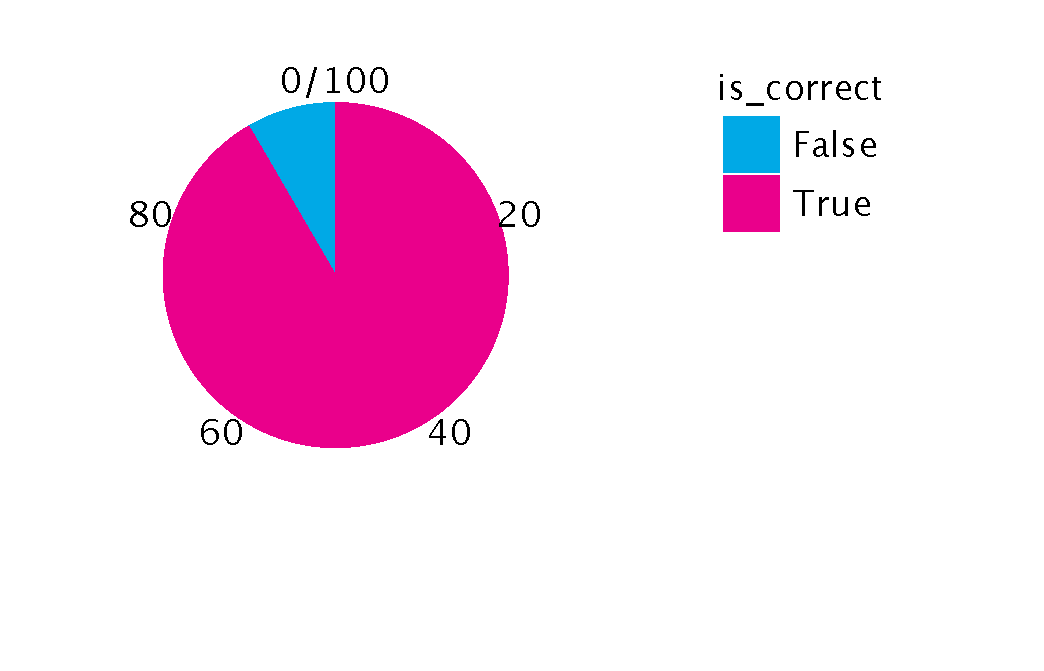
\includegraphics[width=0.7\textwidth]{./figures/correct_camel_background.eps}
    \caption{Boxplot of the two groups}
    \label{fig:boxplot}
\end{figure}

\begin{figure}[h]
    \centering
    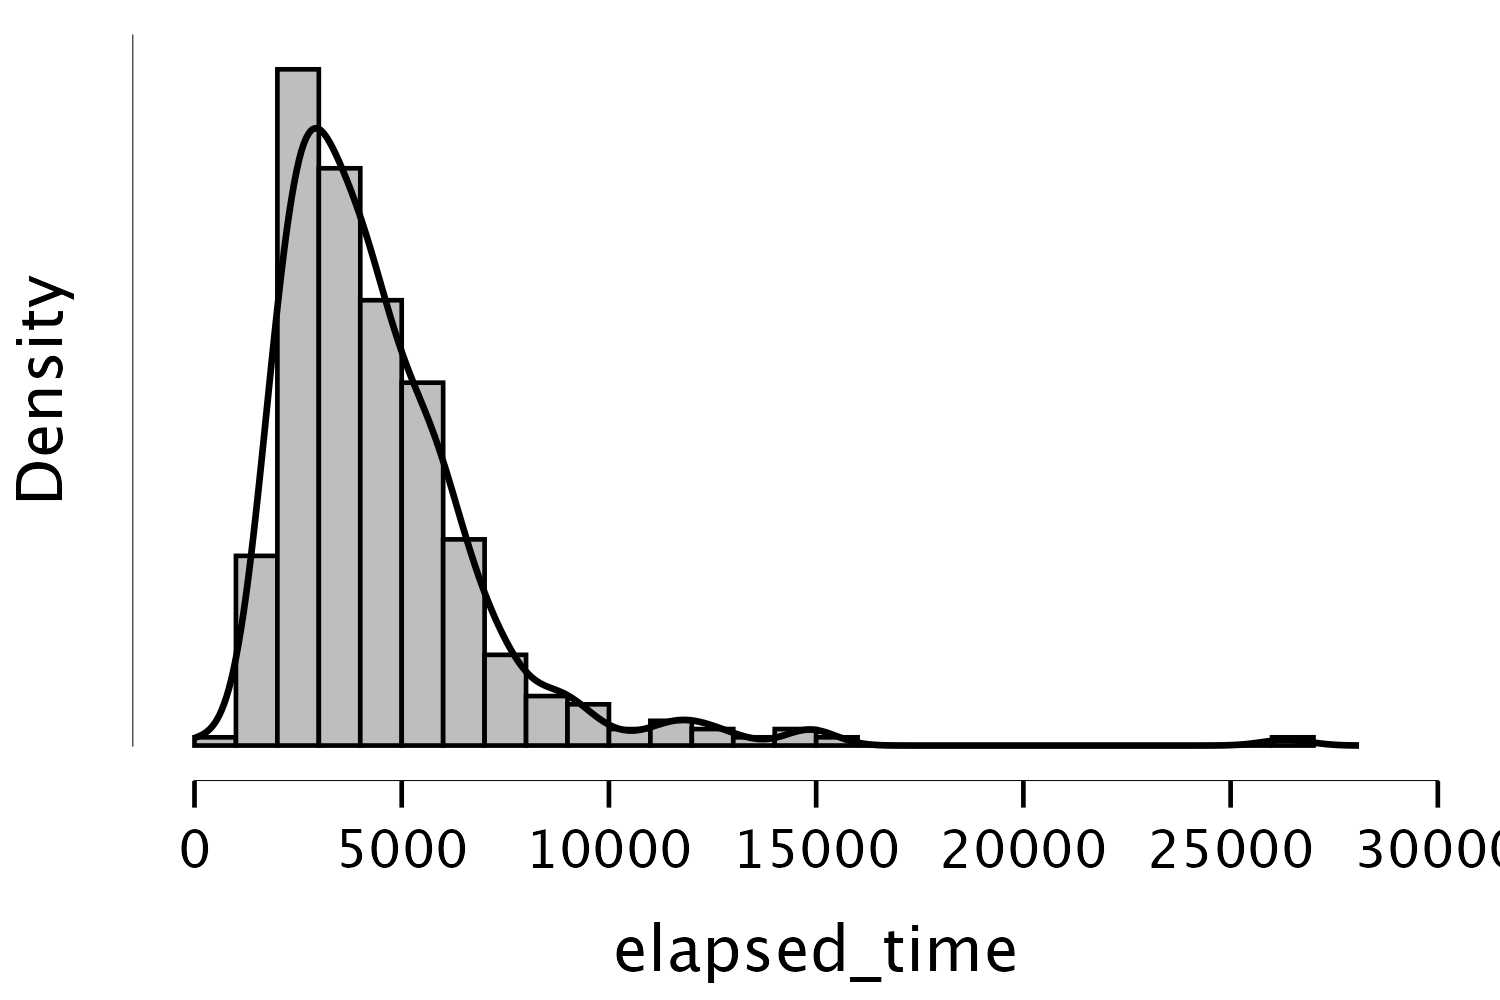
\includegraphics[width=0.7\textwidth]{./figures/correct_camel_distr.png}
    \caption{Boxplot of the two groups}
    \label{fig:boxplot}
\end{figure}

\begin{figure}[h]
    \centering
    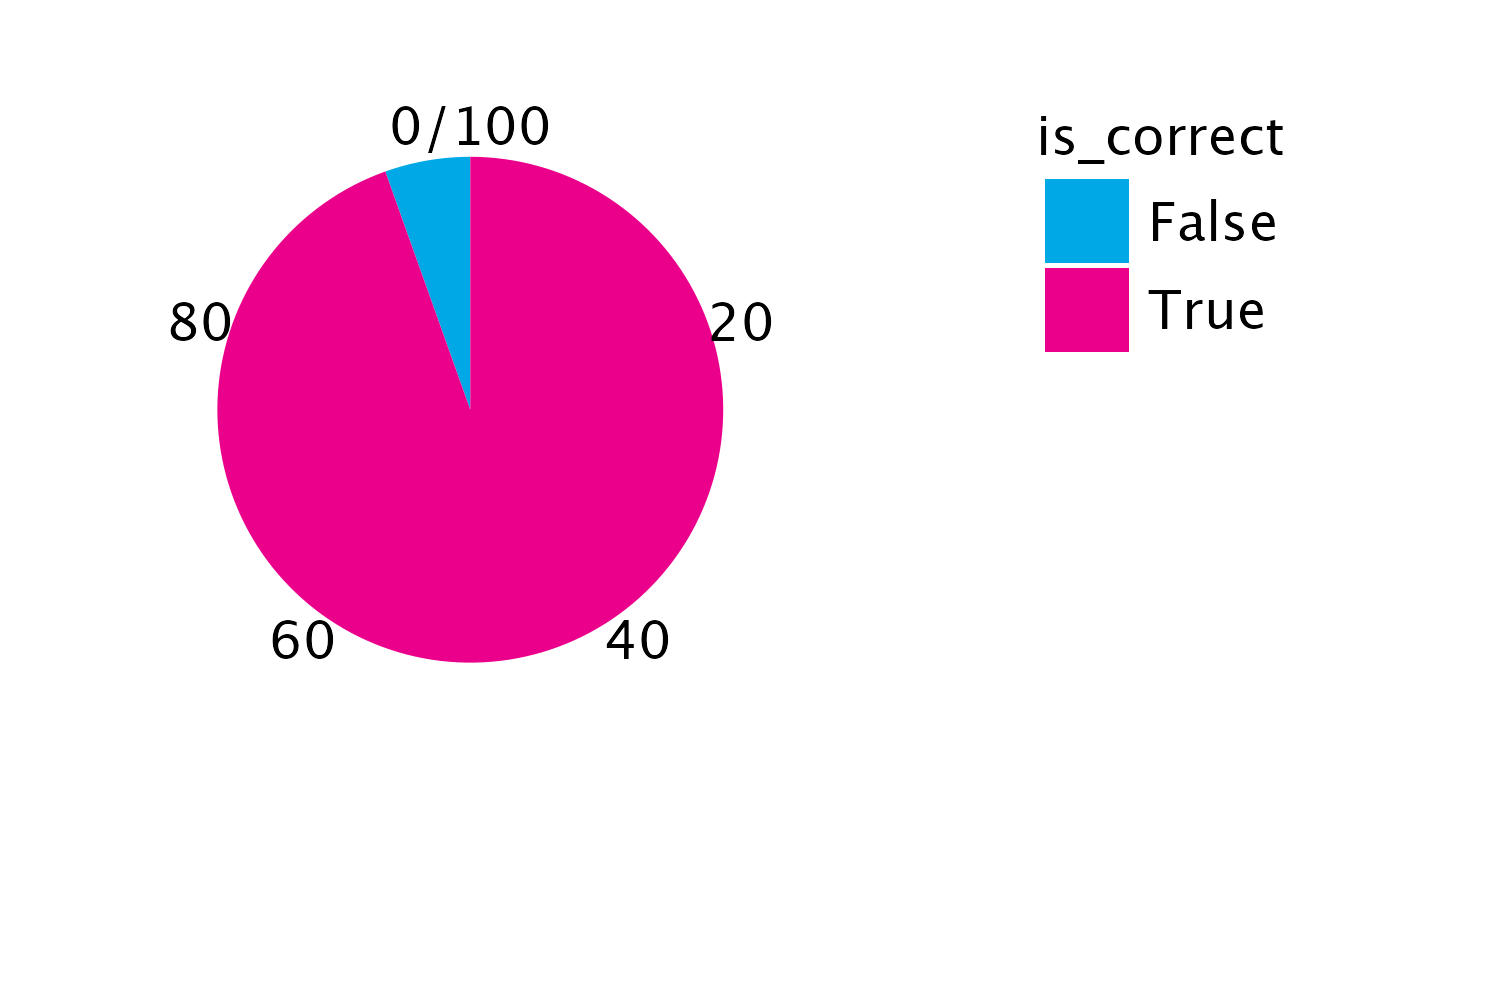
\includegraphics[width=0.7\textwidth]{./figures/correct_camel_noback.png}
    \caption{Boxplot of the two groups}
    \label{fig:boxplot}
\end{figure}

\begin{figure}[h]
    \centering
    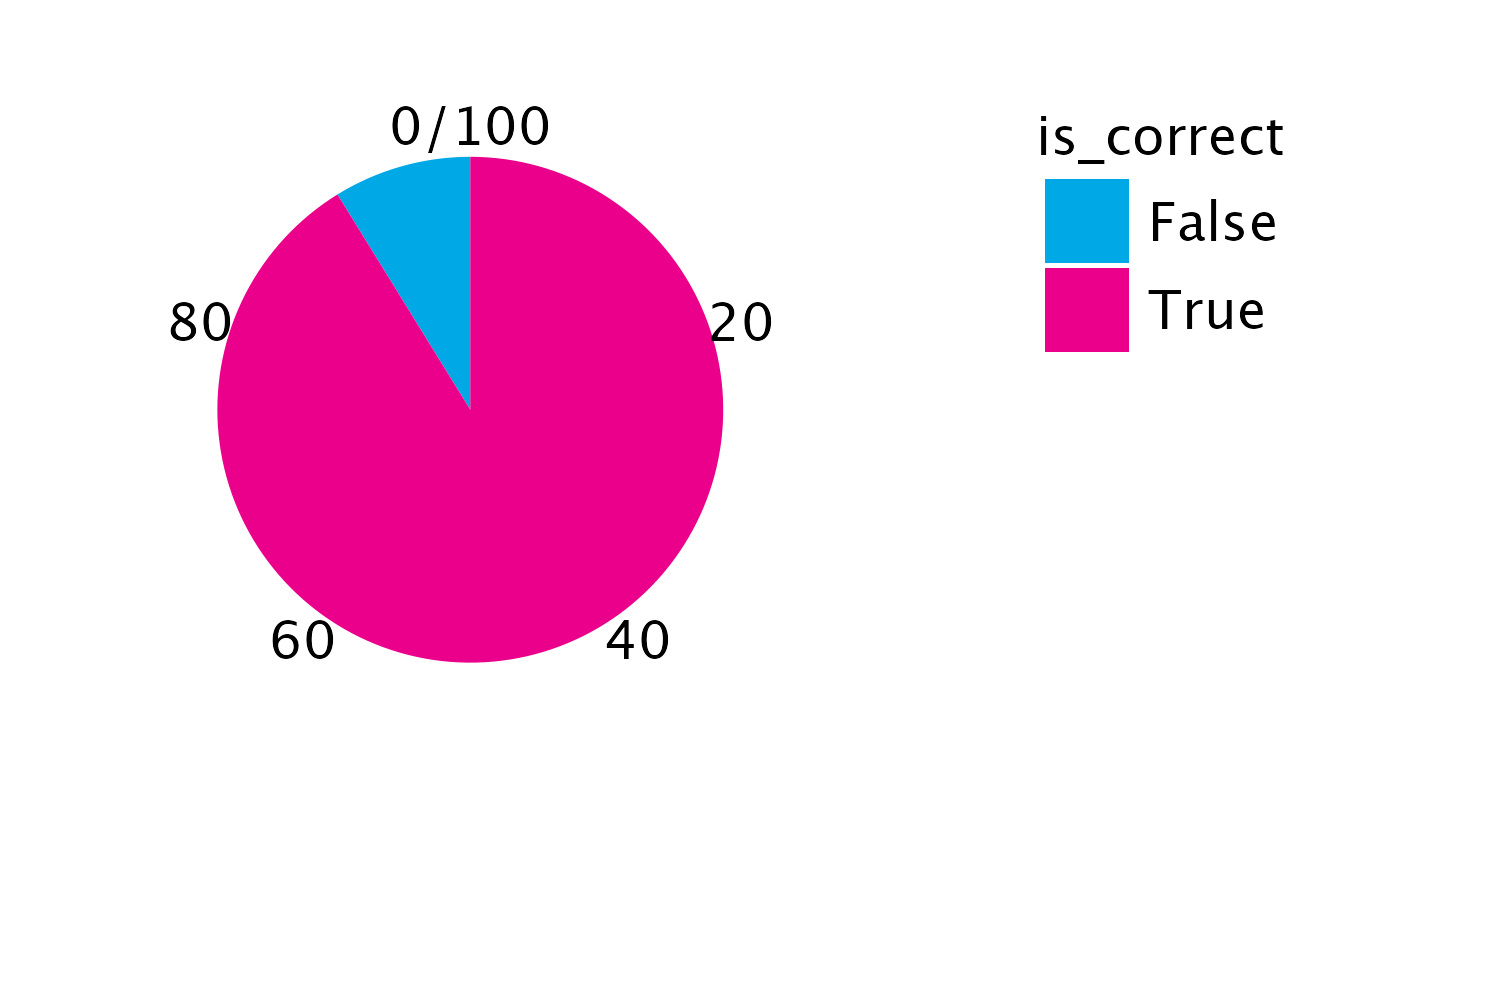
\includegraphics[width=0.7\textwidth]{./figures/correct_keb_backgr.png}
    \caption{Boxplot of the two groups}
    \label{fig:boxplot}
\end{figure}

\begin{figure}[h]
    \centering
    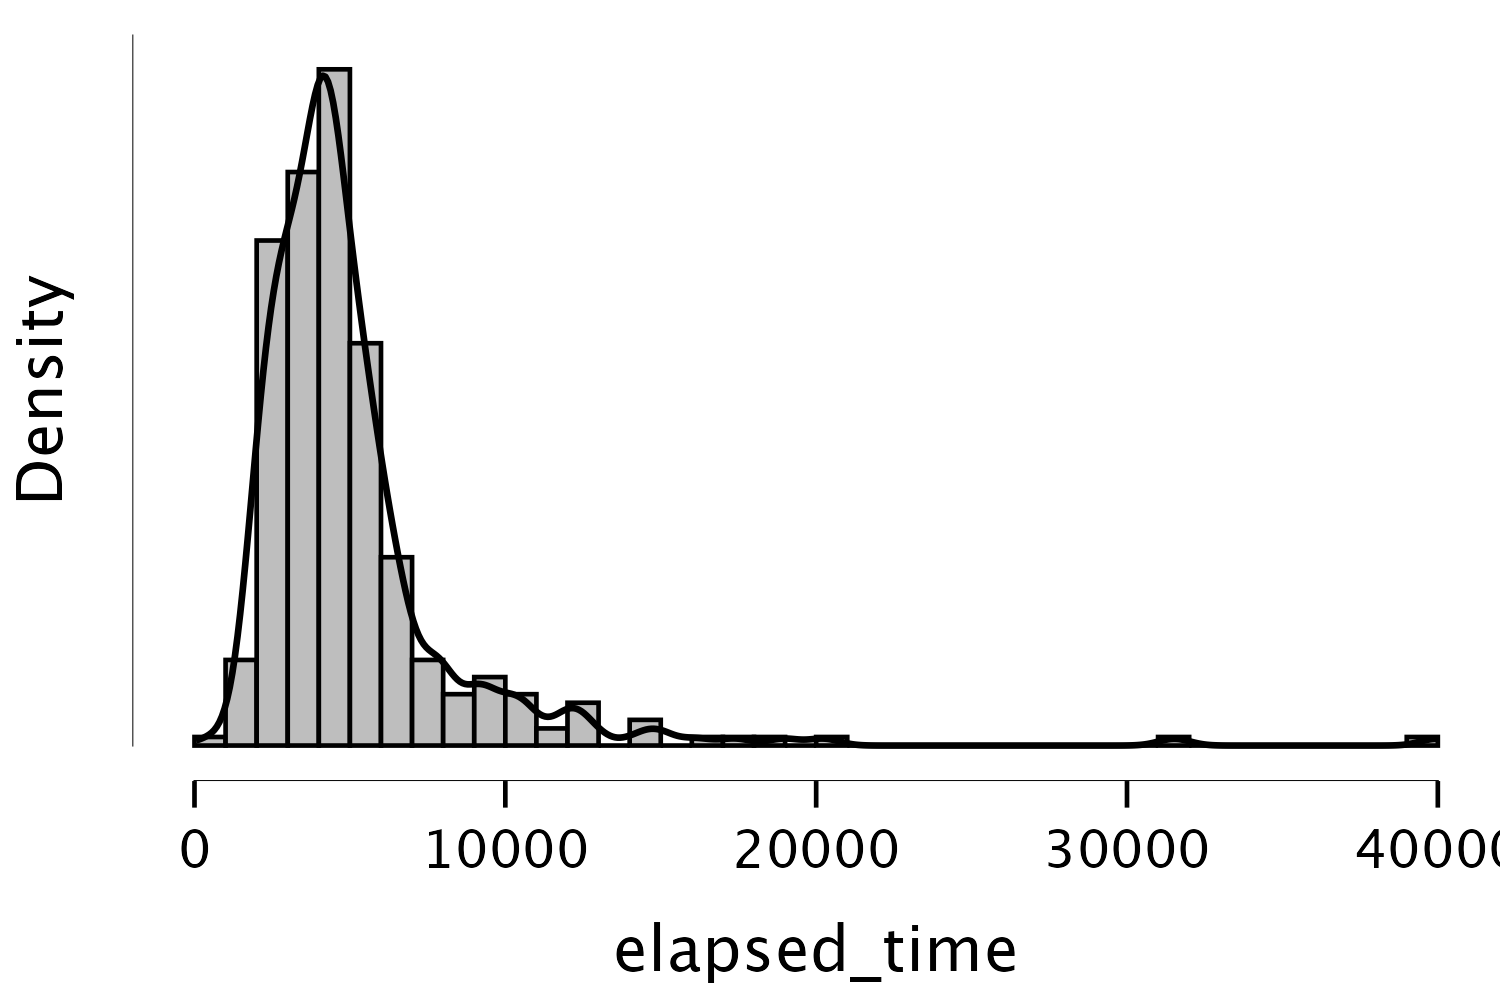
\includegraphics[width=0.7\textwidth]{./figures/correct_kebab_distr.png}
    \caption{Boxplot of the two groups}
    \label{fig:boxplot}
\end{figure}

\begin{figure}[h]
    \centering
    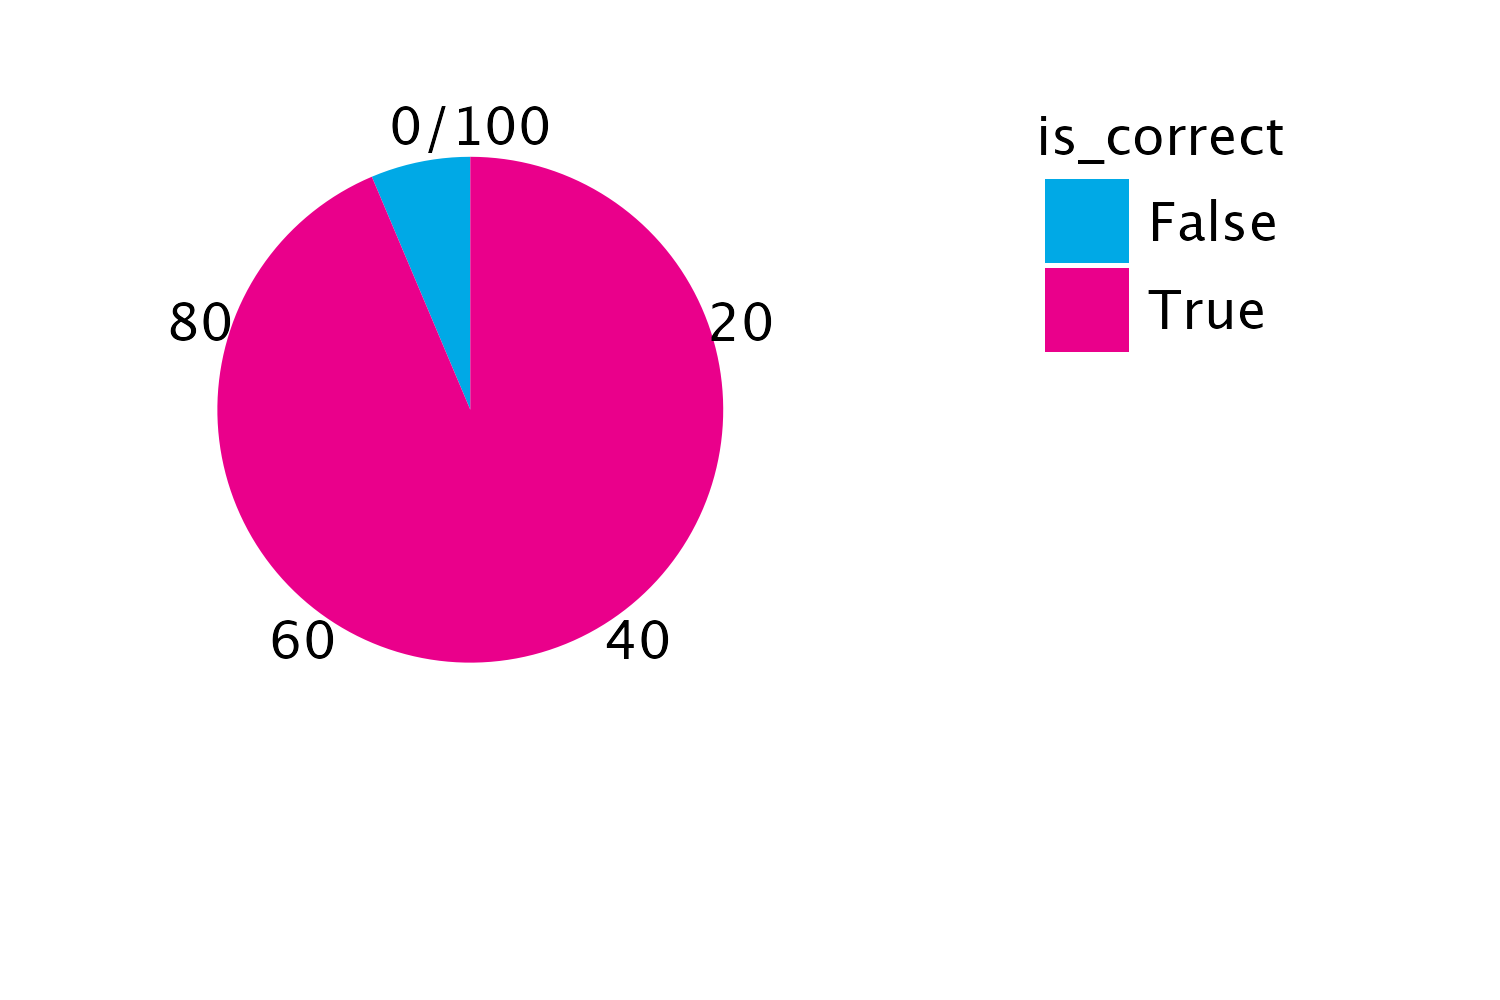
\includegraphics[width=0.7\textwidth]{./figures/correct_kebab_noBack.png}
    \caption{Boxplot of the two groups}
    \label{fig:boxplot}
\end{figure}

\begin{figure}[h]
    \centering
    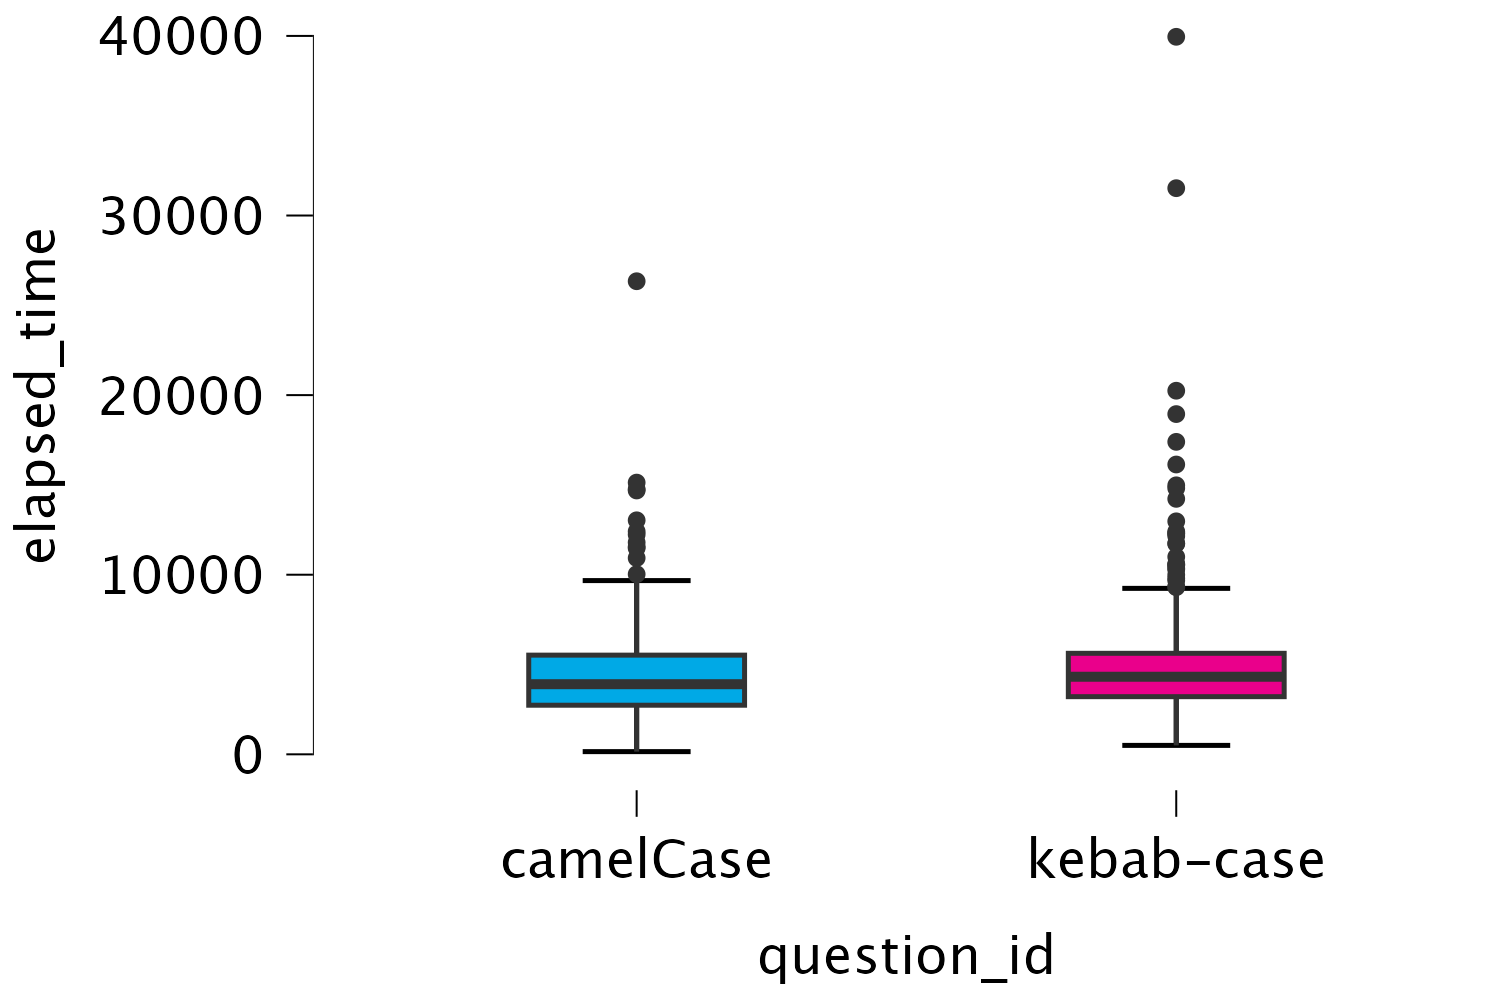
\includegraphics[width=0.7\textwidth]{./figures/elapsed_time_correct.png}
    \caption{Boxplot of the two groups}
    \label{fig:boxplot}
\end{figure}

\subsection{Descriptive Statistics}

Analysis of response times reveals interesting patterns across both identifier styles:

Overall Performance:
- camelCase: Mean = 4442.72ms (SD = 2609.92ms)
- kebab-case: Mean = 5119.94ms (SD = 3691.98ms)

Computer Science Background (CS) vs Non-CS:
CS Participants:
- camelCase: Mean = 3969.64ms (SD = 2113.22ms)
- kebab-case: Mean = 4567.92ms (SD = 3290.78ms)

Non-CS Participants:
- camelCase: Mean = 5296.82ms (SD = 3376.99ms)
- kebab-case: Mean = 6310.29ms (SD = 4330.11ms)

These statistics indicate that:
1. Participants generally performed faster with camelCase
2. CS background correlates with faster response times in both styles
3. Response time variability was higher for kebab-case


\begin{table}[h]
    \centering
    \caption{Descriptive Statistics CSBG}
    \label{tab:descriptiveStatistics}
    {\resizebox{\textwidth}{!}{
            \begin{tabular}{lrrrrrrrr}
                \toprule
                              &            & Mean       & Std. Deviation & Minimum   & Maximum     & 25th percentile & 50th percentile & 75th percentile \\
                \cmidrule[0.4pt]{1-9}
                elapsed\_time & camelCase  & $3969.640$ & $2113.221$     & $150.000$ & $15059.000$ & $2548.250$      & $3511.000$      & $4987.750$      \\
                              & kebab-case & $4567.916$ & $3290.778$     & $328.000$ & $39951.000$ & $3007.250$      & $4007.500$      & $5118.750$      \\
                \bottomrule
            \end{tabular}
        }
    }
\end{table}

\begin{table}[h]
    \centering
    \caption{Descriptive Statistics NON CSBG}
    \label{tab:descriptiveStatistics}
    { \resizebox{\textwidth}{!}{
            \begin{tabular}{lrrrrrrrr}
                \toprule
                              &            & Mean       & Std. Deviation & Minimum    & Maximum     & 25th percentile & 50th percentile & 75th percentile \\
                \cmidrule[0.4pt]{1-9}
                elapsed\_time & camelCase  & $5296.818$ & $3376.998$     & $1744.000$ & $26341.000$ & $3200.250$      & $4419.500$      & $6334.250$      \\
                              & kebab-case & $6310.291$ & $4330.106$     & $1771.000$ & $31522.000$ & $3637.000$      & $4952.500$      & $7584.250$      \\
                \bottomrule
            \end{tabular}
        }}
\end{table}



\begin{table}[h]
    \centering
    \caption{Descriptive Statistics}
    \label{tab:descriptiveStatistics}
    \resizebox{\textwidth}{!}{
        \begin{tabular}{rrrrrrrr}
            \toprule
                       & Mean       & Std. Deviation & Minimum   & Maximum     & 25th percentile & 50th percentile & 75th percentile \\
            \cmidrule[0.4pt]{1-8}
            camelCase  & $4442.718$ & $2609.916$     & $150.000$ & $26341.000$ & $2734.000$      & $3904.000$      & $5522.000$      \\
            kebab-case & $5119.937$ & $3691.977$     & $497.000$ & $39951.000$ & $3209.500$      & $4319.000$      & $5624.000$      \\
            \bottomrule
        \end{tabular}
    }
\end{table}

\subsection{Inferential Statistics}

A paired samples t-test was conducted to compare response times between the two styles:
- t(359) = 3.515, p = 1.000
- Cohen's d = 0.185 (SE = 0.064)

The analysis reveals:
1. The difference in response times is statistically significant
2. The effect size (Cohen's d = 0.185) indicates a small practical difference
3. The results do not support our alternative hypothesis that kebab-case would lead to faster recognition


\begin{table}[h]
    \centering
    \caption{Paired Samples T-Test}
    \label{tab:pairedSamplesT-Test}
    {
        \begin{tabular}{lrrrrrrr}
            \toprule
            Measure 1  &   & Measure 2 & t       & df    & p       & Cohen's d & SE Cohen's d                                                             \\
            \cmidrule[0.4pt]{1-8}
            kebab-case & - & camelCase & $3.515$ & $359$ & $1.000$ & $0.185$   & $0.064$                                                                  \\
            \bottomrule
            \addlinespace[1ex]
            \multicolumn{8}{p{0.8\textwidth}}{\textit{Note.} For all tests, the alternative hypothesis specifies that kebab-case is less than camelCase.} \\
        \end{tabular}
    }
\end{table}


\section{Discussion}
\subsection{Compare Hypotheses with Results}
Contrary to our initial hypothesis, the results show that participants were generally faster at recognizing camelCase identifiers compared to kebab-case. The average difference of approximately 677ms (15.2%) favors camelCase, though with notable individual variation. This finding challenges our initial assumption that explicit separators (as in kebab-case) would facilitate faster recognition.

\subsection{Limitations and Threats to Validity}
Internal Validity Threats:
1. Learning Effects: Despite randomization, participants may have developed pattern recognition strategies during the experiment
2. Fatigue Effects: The 20-question format may have induced fatigue
3. Platform Variations: Different devices and browsers may have affected timing precision

External Validity Threats:
1. Participant Pool: The sample size (n=36) may limit generalizability
2. Artificial Context: The experimental setting differs from real-world code reading
3. Limited Identifier Complexity: Test cases may not fully represent real-world identifier complexity

\subsection{Conclusions}
This study provides evidence that:
1. camelCase identifiers were recognized more quickly than kebab-case identifiers
2. Programming experience significantly influences identifier recognition speed
3. The effect of naming convention on recognition speed, while statistically significant, is relatively small

These findings suggest that contrary to natural language reading patterns, camelCase may offer slight advantages for code identifier recognition. However, the practical significance of these differences is modest enough that other factors (such as team conventions or language standards) may be more important in choosing a naming convention.

Future research could explore:
1. More complex identifier patterns
2. Extended reading tasks beyond single identifier recognition
3. Integration with actual programming tasks


\section{Appendix}

\subsection{Reproduction Package}


\end{document}